\documentclass[hyperref={pdfpagelabels=false},table]{beamer}
\usepackage{Estilo/slides-utfpr}

%\hypersetup{pdfpagemode=FullScreen}   %%% para deixar no modo de tela cheia
\beamertemplatenavigationsymbolsempty   %%% para não mostrar ícones de navegação
% no canto direito inferior

% Nome da disciplina - informação que somente aparece nas propriedades do arquivo PDF
\subject{Trabalho de Conclusão de Curso - UTFPR}

\title[Trabalho de Conclusão de Curso - 2019/1]{Trabalho de Conclusão de Curso -
2019/1}
\subtitle{Navegação de robôs móveis utilizando Lógica \textit{Fuzzy}}
\author[Marcelo Gervazoni Carbonera]{Profa. Orientadora: Dra. Kathya Silvia Collazos
Linares\\
Acadêmico: Marcelo Gervazoni Carbonera}

\institute[UTFPR]{\small{\textbf{Universidade Tecnológica Federal
do Paraná}}\\
Engenharia de Computação\\
\textit{Campus} Pato Branco}
\date{2 de Julho de 2019}

%%%%%%%%%%%%%%%%%%%%%%%%%%%%%%%%%%%%%%%%%%%
%% Para usar subfiguras %%
%%%%%%%%%%%%%%%%%%%%%%%%%%%%%%%%%%%%%%%%%%%
%\usepackage{caption}
\usepackage{subcaption}

%% Bora pro TikZ feraaaa
\usepackage{tikz}
\usetikzlibrary{positioning, patterns, quotes, angles, calc, arrows, shapes}
\usetikzlibrary{arrows.meta}

% Para plotagem
\usepackage{pgfplots}

% para diagrama de transição de estados (SEDs)
\usepackage{dot2texi}

% Para colocar figuras lado a lado
\usepackage{subcaption}
	
% Para calculos
\usepackage{xfp}

% Para matrizes.. (linhas internas)
\usepackage{mleftright}

%%%%%%%%%%%%%%%%%%%%%%%%%%%%%%%%%%%%%%%%%%%%%%%%%%%%%%%%
% Definição de Figuras.
\newcommand{\coordsystwo}[1]{
	\draw[->] (xyz cs:x=0) -- (xyz cs:x=1.5) node[right] {$\hat{X}_{#1}$};
	\draw[->] (xyz cs:y=0) -- (xyz cs:y=1.5) node[above] {$\hat{Y}_{#1}$};
	% The thin ticks
	%\foreach \coo in {-13,-12,...,13}
	%{
	%  \draw (\coo,-1.5pt) -- (\coo,1.5pt);
	%  \draw (-1.5pt,\coo) -- (1.5pt,\coo);
	%  \draw (xyz cs:y=-0.15pt,z=\coo) -- (xyz cs:y=0.15pt,z=\coo);
	%}
	
	% The thick ticks
	%\foreach \coo in {-10,-5,5,10}
	%{
	%\draw[thick] (\coo,-3pt) -- (\coo,3pt) node[below=6pt] {\coo};
	%\draw[thick] (-3pt,\coo) -- (3pt,\coo) node[left=6pt] {\coo};
	%\draw[thick] (xyz cs:y=-0.3pt,z=\coo) -- (xyz cs:y=0.3pt,z=\coo)
	% node[below=8pt] {\coo}; }
	
	% Dashed lines for the points P, Q
	%\draw[dashed] 
	%\draw[dashed] (u) -- (v);
	%\draw[dashed] (-5,7) -- (-5,0) -- (w);
	%\draw[dashed] (3,0) |- (0,5);
	
	% Dots and labels for P, Q
	%\node[fill,circle,inner sep=1.5pt,label={left:$Q(-5,-5,7)$}] at (0,0) {};
	%\node[fill,circle,inner sep=1.5pt,label={above:$P(3,0,5)$}] at (3,5) {};
	% The origin

	% Ponto na origem do sistema de coordenadas
	\node[fill,circle,inner sep=1pt] at (0,0) {};
	
	% Seta para indicar Sistema de coordenadas {X}
	%\node[align=center] at (2,-2) (ori) {\{#1\}};
	%\draw[->,help lines,shorten >=3pt] (ori) .. controls (0.6,-1.3) and (1,-1) ..
	%(0,0,0);
}

\newcommand{\robodiff}{
	% Linhas de baixo, lat esq e dir
	\draw[-, inner sep = 0] (-0.65,-0.75) -- (0.65,-0.75);
	\draw[-, inner sep = 0] (-0.75,-0.65) -- (-0.75,0.5);
	\draw[-, inner sep = 0] (0.75,-0.65) -- (0.75,0.5);
	
	% bordas de baixo
	\draw[-, inner sep = 0] (-0.65,-0.75) -- (-0.75,-0.65);
	\draw[-, inner sep = 0] (0.65,-0.75) -- (0.75,-0.65);
	
	% Retas de cima
	\def\UserL{\fpeval{1.3/(2*cosd(45)+1)}}
	\draw[-, inner sep = 0] (-0.75,0.5) -- (\fpeval{-0.75+\UserL*cosd(45)},
	\fpeval{0.5+\UserL*sind(45)});
	
	\draw[-, inner sep = 0] (0.75,0.5) -- (\fpeval{0.75-\UserL*cosd(45)},
	\fpeval{0.5+\UserL*sind(45)});
	
	\draw[-, inner sep = 0]
	(\fpeval{-0.75+\UserL*cosd(45)},\fpeval{0.5+\UserL*sind(45)}) -- (\fpeval{0.75-\UserL*cosd(45)},
	\fpeval{0.5+\UserL*sind(45)});
	
	% Bola de rolamento
	\filldraw (0,0.65) circle (1.5pt);
	\draw (0,0.65) circle (3pt);
	
	% Desenhar rodas
	\begin{scope}[shift={(-0.75,-0.65)},rotate = 90]
		\draw[rounded corners=2pt] (0,0) rectangle ++(0.8,0.2);
	\end{scope}
	\begin{scope}[shift={(0.75,-0.65)},rotate = 90]
		\draw[rounded corners=2pt] (0,0) rectangle ++(0.8,-0.2);
	\end{scope}
	
	%\draw[dashed, -, inner sep = 0] (-0.75,-0.25) -- (0.75,-0.25);
	
	% Medida R
	\draw[-, inner sep = 0] (+1.2,-0.3) -- ++(0,0.5) node[right] at (+1.4,-0.15)
	{R};
	\draw[-, inner sep = 0] (+1.25,-0.25) -- ++(-0.1,0);
	\draw[-, inner sep = 0] (+1.25,0.15) -- ++(-0.1,0);
	% Medida L
	\draw[-, inner sep = 0] (-0.8,-1) -- (0.8,-1) node[below] at (-0.1,-1.2){L};
	\draw[-, inner sep = 0] (-0.75,-1.05) -- ++(0,0.1);
	\draw[-, inner sep = 0] (0.75,-1.05) -- ++(0,0.1);	
}

\newcommand{\robodiffinercial}{
	\begin{tikzpicture}[scale = 1.3]
		\coordsystwo{I}
		%\draw[-{latex}, shorten >=1.5pt] (0,0) -- (2,2) node[above] at
		%(2.1,0.6){$^{A}Q_{B_{origem}}$};
		% Translação
		\begin{scope}[shift={(2, 2)}]
			%\coordsys{A'}
			% Rotação
			\draw[->] (0.3,0) arc (0:60:0.3);
			\draw[-] (0,0) -- (0.4,0);
			\node at (0.5,0.3) {$\phi$};
			
			% Po 
			\node[color = gray] at (0.1,-0.25) {$P_o$};
			
			\begin{scope}[rotate=60]
				% Ponto Pr
				\node[fill,circle,inner sep=1pt] at (0.6,0) {};
			 	\node[color = gray] at (0.65,0.25) {$P_r$};
			 	\node[color = gray] at (0.3,0.15) {$l$};
			
				\coordsystwo{R}
				\begin{scope}[shift={(0.25,0)},rotate = -90]
					\robodiff
				\end{scope}
				% Flecha até P
				%\draw[-{latex}, shorten >=1.5pt] (0,0) -- (1,2.4) node[right] {$^{B}P$};
				% Ponto em P
				%\node[fill,circle,inner sep=1pt] at (1,2.4) {}; 
				% Definir ponto para desenhar reta
				%\node[align=center,inner sep=0pt] at (1,2.4) (Ponto) {};
			\end{scope}	
		\end{scope}
	% Ponto de {A} para {B}
	%\draw[dashed, -{latex}, shorten >=1pt] (0,0) -- (Ponto) node[above] at (1.5,
	%1.8) {$^{A}P$};
	\end{tikzpicture}
}

\newcommand{\robouniciclo}{
	\begin{scope}[rotate = 90]
	\begin{scope}[shift={(-0.6, -0.15)}]
		\draw[rounded corners=2pt] (0,0) rectangle ++(1.2,0.3);
	\end{scope}
	\end{scope}
}

\newcommand{\robounicicloinercial}{
	\begin{tikzpicture}[scale = 1.3]
		\coordsystwo{I}
		%\draw[-{latex}, shorten >=1.5pt] (0,0) -- (2,2) node[above] at
		%(2.1,0.6){$^{A}Q_{B_{origem}}$};
		% Translação
		\begin{scope}[shift={(2, 2)}]
			%\coordsys{A'}
			% Rotação
			\draw[->] (0.3,0) arc (0:60:0.3);
			\draw[-] (0,0) -- (0.4,0);
			\node at (0.6,0.3) {$\phi$};
			
			\begin{scope}[rotate=60]
				\coordsystwo{R}
				\begin{scope}[rotate = -90]
					\robouniciclo
				\end{scope}
				% Flecha até P
				%\draw[-{latex}, shorten >=1.5pt] (0,0) -- (1,2.4) node[right] {$^{B}P$};
				% Ponto em P
				%\node[fill,circle,inner sep=1pt] at (1,2.4) {}; 
				% Definir ponto para desenhar reta
				%\node[align=center,inner sep=0pt] at (1,2.4) (Ponto) {};
			\end{scope}	
		\end{scope}
	% Ponto de {A} para {B}
	%\draw[dashed, -{latex}, shorten >=1pt] (0,0) -- (Ponto) node[above] at (1.5,
	%1.8) {$^{A}P$};
	\end{tikzpicture}
}

% Definição de bloco e paradinhas para diagramas de bloco
\tikzset{%
    block/.style={scale = 1, draw, fill=white, rectangle, 
            minimum height=2em, minimum width=3em},
    input/.style={inner sep=0pt},       
    output/.style={inner sep=0pt},      
    sum/.style = {scale = 1, draw, fill=white, circle, minimum size=2mm, node
    distance=1.5cm, inner sep=0pt},
    pinstyle/.style = {scale = 1, pin edge={to-,thin,black}}
}

% Definição de subitem para utilizar dentro de itemize
\newcommand{\subitem}[1]{
    {\setlength\itemindent{30pt} \item[$\rightarrow$] #1}
}
%% ============== \begin ====================
\begin{document}

\begin{frame}
	\titlepage
\end{frame}

\section{Navegação de robôs móveis utilizando Lógica \textit{Fuzzy}}

%%%%%%%%%%%%%%%%%%%%%%%%%%%%%%%%%%%%%%%%%%%%%%%%
%%              Plano de Estágio              %%
%%%%%%%%%%%%%%%%%%%%%%%%%%%%%%%%%%%%%%%%%%%%%%%%
\subsection{Estrutura da Apresentação}
\begin{frame}
	\frametitle{Estrutura}
	
	\begin{itemize}
	  \item 1. Introdução
	  \item 2. Objetivos
	  \item 3. Fundamentos Teóricos
	  	\subitem{3.1 Modelo do robô móvel}
	  	\subitem{3.2 Sistemas a Eventos Discretos}
	  	\subitem{3.3 Sistemas Híbridos}
	  	\subitem{3.4 Lógica \textit{Fuzzy} em Controle}
	  \item 4. Materiais e Método
	  \item 5. Desenvolvimento
	  \item 6. Considerações
	\end{itemize}
\end{frame}

\setbeamercovered{transparent}
\subsection{Introdução}
\begin{frame}
	\frametitle{Introdução}
	\begin{block}{Aspectos Qualitativos}
		Arquiteturas:
		\begin{itemize}
		  \item<1,2> Deliberativa.
		  \item<1,3> Reativa.
		  \item<1,4> Híbrida.
		  \item<1,5> Comportamental.
		\end{itemize}
	\end{block}
	
	%\pause
	\begin{overprint}
	\onslide<2>
	\begin{exampleblock}<2>{Deliberativa}
		``Pensar antes de agir''.\\
		Foco no longo prazo.
	\end{exampleblock}
	\onslide<3>
	\begin{exampleblock}<3>{Reativa}
		Reagir rapidamente a estímulos, sem planejar.\\
		Foco no curto prazo.
	\end{exampleblock}
	\onslide<4>
	\begin{exampleblock}<4>{Híbrida}
		Camadas deliberativa e reativa em conjunto.\\
		Desafio: extrair o melhor de cada abordagem.
	\end{exampleblock}
	\onslide<5>
	\begin{exampleblock}<5>{Comportamental}
		Semelhante à arquitetura reativa. \\
		Difere pelo nível de abstração.
	\end{exampleblock}
	\end{overprint}
\end{frame}

\subsection{Objetivos}
\begin{frame}
	\frametitle{Objetivos}
	\begin{exampleblock}{Objetivo Geral}
		\begin{itemize}
		  \item[$\rightarrow$] Construir robô autônomo, sem armazenamento de mapa,
		  capaz de desviar de obstáculos.
		  \item[$\rightarrow$] Comparar qualitativamente: controlador Híbrido e
		  \textit{Fuzzy}.
		\end{itemize}
	\end{exampleblock}
	\pause
	\begin{block}{Objetivos Específicos}
		\begin{itemize}
		  \item[$\rightarrow$] Modelagem.
		  \item[$\rightarrow$] Arquitetura de controle.
		  \item[$\rightarrow$] Implementação física.
		  \item[$\rightarrow$] Implementação do sistema embarcado.
		  \item[$\rightarrow$] Teste e validação.
		\end{itemize}
	\end{block}
\end{frame}
	
\subsection{Fundamentos Teóricos}
\begin{frame}
	\frametitle{Arquitetura comportamental}
	\tikzset{%
    block/.style={scale = 0.9, draw, fill=white, rectangle, 
            minimum height=2em, minimum width=3em},
    input/.style={inner sep=0pt},       
    output/.style={inner sep=0pt},      
    sum/.style = {scale = 0.9, draw, fill=white, circle, minimum size=2mm, node
    distance=1.5cm, inner sep=0pt},
    pinstyle/.style = {scale = 0.9, pin edge={to-,thin,black}}
}

\begin{figure}[h]%
    %\caption{Arbitragem e fusão de comportamentos}%
    \label{fig:subfig2}%
    \centering
    
    \begin{subfigure}[t]{0.5\textwidth}%
	\centering
    
    %\resizebox{0.1\linewidth}{!}{
\begin{tikzpicture}[scale = 0.5, auto, node distance=2cm, on grid, >=latex']%
	\node[block] (C1) {Comportamento 1};
	\node[block, below = 1.6cm of C1] (C2) {Comportamento 2};
	\node[block, below = 1.6cm of C2] (C3) {Comportamento 3};
	\node[input, left = 2cm of C3] (int) {};
	\node[input, below = 1cm of int] (input) {};
	
	\node[right = 2cm of C2, inner sep = 0.2 cm] (sum) {};
	\node[right = 2.22cm of C2, inner sep = 0] (sum1int) {};
	\filldraw (sum1int) circle (0.8pt);
	\node[right = 1.8cm of C2, inner sep = 0] (sum2int) {};
	\node[above = 0.2cm of sum2int, inner sep = 0] (sum2) {};
	\node[output, right = 1cm of sum] (atu) {};
	 
	\coordinate[left = 2cm of C1, inner sep = 0pt] (lC1) {};
	\coordinate[left = 2cm of C2, inner sep = 0] (lC2) {};
	\coordinate[left = 2cm of C3, inner sep = 0] (lC3) {};
	
	\draw [draw,->] (sum) node[below right] {Atuadores} --
	(atu);
	
	\draw [draw,-] (input) node[above right] {Sensores} --
	(lC1);
	\draw [->] (lC1) -- (C1); 
	\draw [->] (lC2) -- (C2);
	\draw [->] (lC3) -- (C3);
	
	\draw [->] (C1) -| node[]{} node[near end] {} (sum);
	\draw [->] (C2) -- (sum);
	\draw [->] (C3) -| node[]{} node[near end] {} (sum);
	
	\draw [-, very thick] (sum1int) -- (sum2);
	
\end{tikzpicture}%    
    %}
    
    \label{fig:subfig1}%
	\caption{Arbitragem}%
	\end{subfigure}%
    ~
    \begin{subfigure}[t]{0.5\textwidth}%
	\centering
	%\resizebox{0.5\linewidth}{!}{
\begin{tikzpicture}[scale = 0.8,auto, node distance=2cm, on grid,
>=latex']%
	\node[block] (C1) {Comportamento 1};
	\node[block, below = 1.6cm of C1] (C2) {Comportamento 2};
	\node[block, below = 1.6cm of C2] (C3) {Comportamento 3};
	\node[input, left = 2cm of C3] (int) {};
	\node[input, below = 1cm of int] (input) {};
	
	\node[sum, right = 2cm of C2] (sum) {+};
	\node[output, right = 1cm of sum] (atu) {};
	 
	\coordinate[left = 2cm of C1, inner sep = 0pt] (lC1) {};
	\coordinate[left = 2cm of C2, inner sep = 0] (lC2) {};
	\coordinate[left = 2cm of C3, inner sep = 0] (lC3) {};
	
	\draw [draw,->] (sum) node[below right] {Atuadores} --
	(atu);
	
	\draw [draw,-] (input) node[above right] {Sensores} --
	(lC1);
	\draw [->] (lC1) -- (C1); 
	\draw [->] (lC2) -- (C2);
	\draw [->] (lC3) -- (C3);
	
	\draw [->] (C1) -| node[]{} node[near end] {} (sum);
	\draw [->] (C2) -- (sum);
	\draw [->] (C3) -| node[]{} node[near end] {} (sum);
	
\end{tikzpicture}%    
%}
	\caption{Fusão}%
	\end{subfigure}%
	
	%\textbf{Fonte: baseado em \citeonline{Livro_Mataric}, p. 167.}
    \label{fig:arbfus}%
\end{figure}

%\begin{tikzpicture}[auto, node distance=2cm, on grid, >=latex']

%\node[input] (input) {};
%\node[input, above = of input] (input1) {};
%\node [sum, right = of input] (sum) {};
%\node [block, right = of sum] (controller) {$K(s)$};
%\node [sum, right = of controller] (sum1) {};
%\node [block, right = of sum1] (filterinv) {$H^{-1}(s)$};
%\node [block, right = 2.5cm of filterinv] (system) {$G(s)$};
%\node [output, right = of system] (output) {};
%\node [output, above = of output] (output1) {};
%\node [block, above = of controller] (delay) {$D(s)$};
%\node [sum, below = of sum1] (sum2) {};
%\node [block] (filter) at (sum2-|filterinv) {$H(s)$};

%\draw [draw,->] (input) node[above right] {$s_{i-1}$} -- (sum);
%\draw [->] (sum) -- node {$e_{i}$} (controller);
%\draw [->] (controller) -- node {} (sum1);
%\draw [->] (sum1) -- node[name=xi] {$\xi_{i}$} (filterinv);
%\draw [->] (filterinv) -- node[name=u, pos=.3] {$u_{i}$} (system);
%\draw [->] (system) -- (output) node [name=q, above left] {$q_{i}$};

%\draw [->] ([xshift=-5mm]q.south) |- (filter);
%\draw [->] (filter) -- node {} (sum2);
%\draw [draw,<-] (sum2) -- ++(90:.6cm) node[above]{$L_i+r_i$};

%\draw [->] (sum2) -| node[pos=0.99, right] {$-$} 
%    node [pos=.25, above] {$\tilde{s}_i$} (sum);

%\draw [draw,->] (input1) node[above right] (ui-1) {$u_{i-1}$} -- (delay);
%\draw [->] (delay) -| node[] {} 
%    node [near end] {} (sum1);

%\draw [->] (u.east|-system) |-  
%    (output1) node[above left] (ui) {$u_i$};

%\node[text=red, above left= 5mm and 6mm of ui.west] (veh) {vehicle $i$};
%\draw[red, dashed]
% (veh.east)-|(ui.west)|-([yshift=-3mm]filter.south)-|(ui-1.east)|-(veh.west);

%\end{tikzpicture}
\end{frame}

\begin{frame}
	\frametitle{Comportamentos como campos potenciais}
	\begin{figure}[h]%
    %\caption{Comportamentos definidos por campos potenciais}%
    %\label{fig:subfig2}%
    \centering
    
    \begin{subfigure}[t]{0.5\textwidth}%
	\centering
    
    %\resizebox{0.1\linewidth}{!}{
\begin{tikzpicture}[scale = 0.7,auto, node distance=2cm, on grid, >=latex']%
\begin{axis}[view={0}{90}, axis equal image]
	\addplot3[darkgray, domain=-2:2, y domain=-2:2, 
		quiver={
			u={-x}, v={-y},
			scale arrows=0.2}, ->,samples=21,
			y filter/.append
			code={\pgfmathparse{(sqrt(x^2+y^2)>1.8)||(sqrt(x^2+y^2)<0.1||(sqrt(x^2+y^2)>1))
			? nan : y}}] {0};
			
	\addplot3[darkgray, domain=-2:2, y domain=-2:2, 
		quiver={
			u={-x/(sqrt(x^2+y^2))}, v={-y/(sqrt(x^2+y^2)},
			scale arrows=0.2}, ->,samples=21,
			y filter/.append
			code={\pgfmathparse{(sqrt(x^2+y^2)>1.8)||(sqrt(x^2+y^2)<0.1||(sqrt(x^2+y^2)<=1))
			? nan : y}}] {0};
			
	\addplot3[gray, domain=-1.905:1.905, y domain=-1.905:1.905, 
		quiver={
			u={-x}, v={-y},
			scale arrows=0.2}, ->,samples=20,
			y filter/.append
			code={\pgfmathparse{(sqrt(x^2+y^2)>1.8)||(sqrt(x^2+y^2)<0.1)||(sqrt(x^2+y^2)>1)
			? nan : y}}] {0};
			
	\addplot3[gray, domain=-1.905:1.905, y domain=-1.905:1.905, 
		quiver={
			u={-x/(sqrt(x^2+y^2))}, v={-y/(sqrt(x^2+y^2))},
			scale arrows=0.2}, ->,samples=20,
			y filter/.append
			code={\pgfmathparse{(sqrt(x^2+y^2)>1.8)||(sqrt(x^2+y^2)<0.1)||(sqrt(x^2+y^2)<=1)
			? nan : y}}] {0};
			
\end{axis}
\end{tikzpicture}%    
    %}
    
    %\label{fig:subfig1}%
	\caption{Comportamento ``Ir Para Objetivo''}%
	\end{subfigure}%
    ~
    \begin{subfigure}[t]{0.5\textwidth}%
	\centering
	%\resizebox{0.5\linewidth}{!}{
\begin{tikzpicture}[scale = 0.7,auto, node distance=2cm, on grid,
>=latex']%
\begin{axis}[view={0}{90}, axis equal image]
\addplot3[darkgray, domain=-2:2, y domain=-2:2, 
		quiver={
			u={-x/2 + x/(sqrt(x^2+y^2))}, v={-y/2 + y/(sqrt(x^2+y^2))}, scale
			arrows=0.25}, ->,samples=21, 
			y filter/.append
			code={\pgfmathparse{(sqrt(x^2+y^2)>1.8)||(sqrt(x^2+y^2)<0.1) ? nan : y}}] {0};

\addplot3[gray, domain=-1.905:1.905, y domain=-1.905:1.905, 
		quiver={
			u={-x/2 + x/(sqrt(x^2+y^2))}, v={-y/2 + y/(sqrt(x^2+y^2))},
			scale arrows=0.25}, ->,samples=20,
			y filter/.append
			code={\pgfmathparse{(sqrt(x^2+y^2)>1.8)||(sqrt(x^2+y^2)<0.1) ? nan : y}}]
			{0};

\end{axis}
\end{tikzpicture}%    
%}
	\caption{Comportamento ``Evitar Obstáculo''}%
	\end{subfigure}%
	
	%\textbf{Fonte: baseado em \citeonline{book:arkin}, p. 146 e 148}
    \label{fig:campovet}%
\end{figure}
\end{frame}

\begin{frame}
	\begin{block}{Mínimos locais}
		\begin{itemize}
		  \item Existência de mínimos locais depende da disposição e formato de
		  obstáculos.
		  \item Um comportamento ``Seguidor de parede'' pode ser criado a fim de
		  contornar obstáculos.
		\end{itemize}
	\end{block}
\end{frame}

% Mínimos locais (obstáculos côncavos e convexos).
% Comportamento Seguir parede.

\begin{frame}
	\frametitle{Modelo Cinemático}
	%\begin{tikzpicture}[x=0.5cm,y=0.5cm,z=0.3cm,>=stealth]
% The axes

\begin{figure}[h]
\centering
%\caption{Modelos uniciclo e diferencial}
\label{fig:modelo}
	 \begin{subfigure}[t]{0.5\textwidth}%
		\centering
		\robounicicloinercial
		\label{fig:uniciclo}%
		\caption{Uniciclo}%
		\end{subfigure}%
    	~
    \begin{subfigure}[t]{0.5\textwidth}%
		\centering
		\robodiffinercial
		\label{fig:diff}%
		\caption{Diferencial}%
		\end{subfigure}%
		%\textbf{Fonte: baseado em \citeonline{Livro_Siegwart}, p. 49 e 54.}
\end{figure}

%\begin{tikzpicture}[x=0.5cm,y=0.5cm,z=0.3cm,>=stealth]
\end{frame}

\begin{frame}
	\begin{tabular}{cl}  
    	\begin{tabular}{c}
			\robounicicloinercial
		\end{tabular}
		& \begin{tabular}{l}
			\parbox{0.5\linewidth}{
				$
					\left \{ \begin{matrix} \dot{x} &= v\cos{\phi} \\ \dot{y} &= v\sin{\phi} \\
					\dot{\phi} &= \omega \end{matrix} \right.
				$
				
				$
					\mleft[ 
					\begin{array}{c c}
					\dot{x} \\ \dot{y} \\ \dot{\phi}
					\end{array}
					\mright] = \mleft[
					\begin{matrix}
		  				\cos{\phi} & 0 \\
		  				\sin{\phi} & 0 \\
		  				0 & 1 \\
					\end{matrix}
					\mright] \mleft[ 
					\begin{array}{c c}
					v \\ \omega
					\end{array}
					\mright]
				$
			}
		\end{tabular}\\
	\end{tabular}
\end{frame}

\begin{frame}
	\begin{tabular}{cl}
    	\begin{tabular}{c}
    		\parbox{0.5\linewidth}{
			$
				\left \{ \begin{matrix} \dot{x} = \frac{R}{2}(\omega_l +
				\omega_r)\cos{\phi}
				\\
				\dot{y} = \frac{R}{2}(\omega_l +
				\omega_r)\sin{\phi}
				\\
				\dot{\phi} = \frac{R}{L}(\omega_r -
				\omega_l) \end{matrix} \right.
			$
			}
		\end{tabular}
		\begin{tabular}{l}
			\robodiffinercial
		\end{tabular}
	\end{tabular}
\end{frame}

\begin{frame}
	\frametitle{Estabelecendo vínculo entre os modelos}
	\vfill
	\begin{tabular}{cl}  
		\begin{tabular}{c}
			\parbox{0.5\linewidth}{
			$
				\left \{ \begin{matrix} \dot{x} = \frac{R}{2}(\omega_l +
				\omega_r)\cos{\phi}
				\\
				\dot{y} = \frac{R}{2}(\omega_l +
				\omega_r)\sin{\phi}
				\\
				\dot{\phi} = \frac{R}{L}(\omega_r -
				\omega_l) \end{matrix} \right.
			$
			}
		\end{tabular}
		& \begin{tabular}{l}
			\parbox{0.5\linewidth}{
			$
				\left \{ \begin{matrix} \dot{x} &= v\cos{\phi} \\ \dot{y} &= v\sin{\phi} \\
				\dot{\phi} &= \omega \end{matrix} \right.
			$
			}
		\end{tabular}
	\end{tabular}
	\vfill
	\begin{exampleblock}{\centerline{Equivalência entre modelos}}
	\centerline{
	$
	\begin{matrix}
		\omega_l = \frac{2v - L\omega}{2R} 
		\\
		\\	
		\omega_r = \frac{2v + L\omega}{2R}
	\end{matrix}
	$
	}
	\end{exampleblock}
	\vfill
\end{frame}

\setbeamercovered{invisible}
\begin{frame}
	\frametitle{O modelo de integrador único}
	\begin{tabular}{cl}
    	\begin{tabular}{c}
    		\hspace{-1cm}
    		\parbox{0.5\linewidth}{
    		\vspace{1.3cm}
    		\begin{itemize}
    		\item<1->[]
			$
				\left \{ \begin{matrix} x' = x_o + l\cos{\phi}
				\\
				y' = y_o + l\sin{\phi}
				\end{matrix} \right.
			$
			\item<2->[]
			$
				\left \{ \begin{matrix} \dot{x'} = \dot{x_o} - \dot{\phi}l\sin{\phi} =
				v\cos{\phi} - l\omega\sin{\phi}
				\\
				\dot{y'} = \dot{y_o} + \dot{\phi}l\cos{\phi} = v\sin{\phi} +
				l\omega\cos{\phi} \end{matrix} \right.
			$
			\item<3->[]
			\mbox{\small
			$
				\mleft[ 
				\begin{array}{c c}
				\dot{x'} \\ \dot{y'}
				\end{array}
				\mright] = \mleft[
				\begin{matrix}
		  			\cos{\phi} & -\sin{\phi} \\
		  			\sin{\phi} & \cos{\phi} \\
				\end{matrix}
				\mright] \mleft[
				\begin{matrix}
		  			1 & 0 \\
		  			0 & l \\
				\end{matrix}
				\mright] \mleft[ 
				\begin{array}{c c}
				v \\ \omega
				\end{array}
				\mright]
			$
			}
			\item<4->[]
			\mbox{\small
			$
				\mleft[ 
				\begin{array}{c c}
				v \\ \omega
				\end{array}
				\mright] = \mleft[
				\begin{matrix}
					1 & 0 \\
		  			0 & \frac{1}{l} \\
				\end{matrix}
				\mright] \mleft[
				\begin{matrix}
		  			\cos{\phi} & \sin{\phi} \\
		  			-\sin{\phi} & \cos{\phi} \\
				\end{matrix}
				\mright] \mleft[ 
				\begin{array}{c c}
					\dot{x'} \\ \dot{y'}
				\end{array}
				\mright]
			$
			}
			\item<5>[]
			\mbox{\small
			$
				\mleft[ 
				\begin{array}{c c}
					\omega_l \\ \omega_r
				\end{array}
				\mright] = \mleft[
				\begin{matrix}
		  			\frac{1}{R} & \frac{-L}{2R} \\
		  			\frac{1}{R} & \frac{L}{2R} \\
				\end{matrix}
				\mright] \mleft[
				\begin{matrix}
		  			1 & 0 \\
		  			0 & \frac{1}{l} \\
				\end{matrix}
				\mright] \mleft[
				\begin{matrix}
		  			\cos{\phi} & \sin{\phi} \\
		  			-\sin{\phi} & \cos{\phi} \\
				\end{matrix}
				\mright] \mleft[ 
				\begin{array}{c c}
					\dot{x'} \\ \dot{y'}
				\end{array}
				\mright]
			$
			}
			\end{itemize}
			}
		\end{tabular}
		\begin{tabular}{l}
			\hspace{1cm}
			\robodiffinercial
		\end{tabular}
	\end{tabular}
\end{frame}

\begin{frame}
	\frametitle{Sistemas a Eventos Discretos}
	\begin{block}{Definição}
		\begin{itemize}
		  \item Sistema Dinâmico.
		  \item Estados discretos.
		  \item Eventos assíncronos provocam transições instantâneas de estado.
		  \item Arbitragem!
		\end{itemize}
	\end{block}
	
	\vspace{-0.15cm}
	\tikzset{%
    block/.style={draw, fill=white, rectangle, 
            minimum height=2em, minimum width=3em},
    input/.style={inner sep=0pt},       
    output/.style={inner sep=0pt},      
    sum/.style = {draw, fill=white, circle, minimum size=2mm, node
    distance=1cm, inner sep=0pt},
    pinstyle/.style = {pin edge={to-,thin,black}}
}

\begin{figure}[h]
    \centering
\begin{tikzpicture}[scale = 1, ->,auto,node distance =4 cm and 5cm ,on grid,
>=latex',
state/.style ={scale = 1, circle, draw, minimum width =0.7cm},
finalstate/.style ={scale = 1, circle, draw, minimum width =0.7cm}]

	\node[finalstate, double, double distance=1pt, outer sep = 1pt] (x) {$x$};
	\node[state, right = 3.4cm of x] (y) {$y$};
	\node[finalstate, double, double distance = 1pt, outer sep = 1pt, below right
	= 2.5cm of x] (z) {$z$};
	
	\path[->] (x) edge node[below left] {$g$} (z);
	\path[->] (z) edge node[below right] {$a,g$} (y);
	\path[->] (y) edge node[above] {$a$} (x);
	
	\draw (x) to [out=60,in=120,looseness=6] node[above] {$a$} (x);
	\draw (y) to [out=60,in=120,looseness=6] node[above] {$b$} (y);
	\draw (z) to [out=240,in=300,looseness=6] node[below] {$b$} (z);
	
	% Input
	\coordinate[left = 1cm of x, inner sep = 0pt] (input) {};
	\path[->] (input) edge (x);
\end{tikzpicture}%    
\end{figure}
\end{frame}

\begin{frame}
	\frametitle{Controle Supervisório}
	\begin{block}{Definição}
		\begin{itemize}
		  \item Captura eventos observáveis.
		  \item Permite ou suprime eventos passíveis de ocorrência.
		\end{itemize}
	\end{block}
	
	\vspace{0.3cm}
	\tikzset{%
    block/.style={scale = 1, draw, fill=white, rectangle, 
            minimum height=2em, minimum width=3em},
    input/.style={inner sep=0pt},       
    output/.style={inner sep=0pt},      
    sum/.style = {scale = 1, draw, fill=white, circle, minimum size=2mm, node
    distance=1.5cm, inner sep=0pt},
    pinstyle/.style = {scale = 1, pin edge={to-,thin,black}}
}

\begin{figure}[h]%
    \centering
\begin{tikzpicture}[scale = 1, auto, node distance=2cm, on grid,
>=latex']%
	\node[block] (P) {Planta};
	\node[block, below = 1.8cm of P] (S) {Supervisor};
	
	\coordinate[left = 2cm of S, inner sep = 0pt] (int1) {};
	\coordinate[right = 2cm of P, inner sep = 0pt] (int2) {};
	
	\draw [->] (P) -| (int2) node[below right] {Eventos Observados} |- (S);
	\draw [->] (S) -| (int1) node[above left] {Eventos Desabilitados} |- (P);
	
	%node[above] {$a$}
\end{tikzpicture}%    
\end{figure}


\end{frame}

\begin{frame}	
	\frametitle{Automatos Temporizados com guarda}
	
	\begin{exampleblock}{\textit{clocks}}
		\begin{itemize}
		  \item ``Contador'': associado a tempo.
		  \item Definido por uma função linear ($\dot{x} = 1$).
		\end{itemize}
	\end{exampleblock}
	
	\begin{block}{Função de transição}
		\begin{itemize}
		  \item Transições: (Estado, Evento) $\rightarrow$ (Estado)
		  \item Transições Temporizadas: (Guardas, Evento, \textit{Reset})
		  $\rightarrow$ (Estado)
		  \subitem{Guardas: condições nas variáveis contínuas.}
		  \subitem{\textit{Reset}: conjunto de variáveis \textit{clock} às quais
		  deve-se atribuir valor zero.}
		\end{itemize}
	\end{block}
	
\end{frame}

\begin{frame}
	\vspace{-0.6cm}
	\tikzset{%
    block/.style={draw, fill=white, rectangle, 
            minimum height=2em, minimum width=3em},
    input/.style={inner sep=0pt},       
    output/.style={inner sep=0pt},      
    sum/.style = {draw, fill=white, circle, minimum size=2mm, node distance=1.5cm, inner sep=0pt},
    pinstyle/.style = {pin edge={to-,thin,black}}
}

\newcommand{\diagum}{
\begin{tikzpicture}[scale = 1,->,auto ,node distance =4 cm and 5cm , on grid,
>=latex' ,
state/.style ={scale = 0.9, circle, draw, minimum width =0.7cm},
finalstate/.style ={scale = 0.9, circle, draw, minimum width =0.7cm}]
	
	\node[state] (a) {0};
	\node[state, above right = 2.5cm of a] (b) {1};
	\node[state, below right = 2.5cm of b] (c) {2};
	\node[state, below left = 2.5cm of c] (d) {3};
	
	\path[->] (a) edge node[above left] {$\emptyset; a; c_1$} (b);
	\small
	\path[->] (b) edge node[above right] {$0<c_1<1; a; c_1$} (c);
	\normalsize
	\path[->] (c) edge node[below right] {$c_1<1; b; \emptyset$} (d);
	\draw (b) to [out=120,in=60,looseness=6] node[above] {$c_1\geq1;a;c_1$} (b);
	
	% Input
	\coordinate[left = 1cm of a, inner sep = 0pt] (input) {};
	\path[->] (input) edge (a);
\end{tikzpicture}%
}

\newcommand{\diagdois}{
\begin{tikzpicture}[->,auto ,node distance =4 cm and 5cm ,on grid ,
>=latex' ,
state/.style ={scale = 0.9, circle, draw, minimum width =0.7cm},
finalstate/.style ={scale = 0.9, circle, draw, minimum width =0.7cm}]

	\node[state] (a) {0};
	\node[state, above right = 2.5cm of a] (b) {1};
	\node[state, below right = 2.5cm of b, align = center] (c) {2 \\ $c_1<1$};
	\node[state, below left = 2.5cm of c] (d) {3};
	
	\path[->] (a) edge node[above left] {$\emptyset; a; c_1$} (b);
	\small
	\path[->] (b) edge node[above right] {$0<c_1<1; a; c_1$} (c);
	\normalsize
	\path[->] (c) edge node[below right] {$\emptyset; b; \emptyset$} (d);
	\draw (b) to [out=120,in=60,looseness=6] node[above] {$c_1\geq1;a;c_1$} (b);
	
	% Input
	\coordinate[left = 1cm of a, inner sep = 0pt] (input) {};
	\path[->] (input) edge (a);	
\end{tikzpicture}%
}

% Figura
\begin{figure}[h]
\centering
%\caption{Exemplos de diagramas de transição para autômatos temporizados com
%guarda} 
	%\label{fig:ATG}
	\begin{subfigure}[t]{0.5\textwidth}%
		\centering
		\diagum%
		%\label{fig:guardadiag1}%
		%\caption{Exemplo 1}%
		\end{subfigure}%
    	~
    	\begin{subfigure}[t]{0.5\textwidth}%
		\centering
		\diagdois%
		%\label{fig:guardadiag2}%
		%\caption{Exemplo 2}%
		\end{subfigure}%
		
		%\textbf{Fonte: baseado em \citeonline{book:SED}, p. 301.}
\end{figure}
	\pause
	\begin{exampleblock}{Invariante}
		Evita \textit{deadlock} por tempo ao forçar transição!
	\end{exampleblock}
\end{frame}

\begin{frame}
	\frametitle{Sistemas Híbridos}
	\begin{block}{Definição}
		\begin{itemize}
		  \item Estados formados por tuplas (q,\textbf{x}).
		  \subitem{q: Estados discretos}.
		  \subitem{\textbf{x}: Estados contínuos}.
		  \item Autômato híbrido extende o autômato temporizado com guardas.
		  \item Estados são chamados ``\textbf{modos de operação}'', pois alteram a
		  dinâmica do sistema.
		\end{itemize}
	\end{block}
	\pause
	\begin{exampleblock}{Arbitragem}
		Chaveamento de dinâmicas (controladores).
	\end{exampleblock}
\end{frame}

\begin{frame}
	\tikzset{%
    block/.style={scale = 1.2,draw, fill=white, rectangle, 
            minimum height=2em, minimum width=3em},
    input/.style={inner sep=0pt},       
    output/.style={inner sep=0pt},      
    sum/.style = {scale = 1.2,draw, fill=white, circle, minimum size=2mm, node
    distance=1.5cm, inner sep=0pt},
    pinstyle/.style = {scale = 1.2,pin edge={to-,thin,black}}
}

\begin{figure}[h]%
    %\caption{Controlador Híbrido}%
    %\label{fig:subfig2}%
    \centering
    
\resizebox{7cm}{!}{
\begin{tikzpicture}[scale = 1,auto, node distance=2cm, on grid, >=latex']%
	\node[block] (C1) {Controlador Supervisório};
	\node[block, below = 2.7cm of C1] (C2) {Interface};
	\node[block, below = 2.7cm of C2] (C3) {Controlador de Variável Contínua};
	\node[block, below = 2.7cm of C3] (C4) {Sistema};
	
	\coordinate[left = 0.5cm of C1.south, inner sep = 0pt] (c1vai) {};
	\coordinate[right = 0.5cm of C1.south, inner sep = 0pt] (c1vem) {};
	\coordinate[right = 0.5cm of C2.north, inner sep = 0pt] (c2vai) {};
	\coordinate[left = 0.5cm of C2.north, inner sep = 0pt] (c2vem) {};
	\draw [draw,->] (c1vai.south) -- (c2vem.north);
	\draw [draw,->] (c2vai.north) -- (c1vem.south);
	
	\node[below = 0.7cm of C1.south, inner sep = 0pt] (comand) {};
	\node (com1) {};
	\node[left = 1.6cm of comand, inner sep = 0pt] (com) {Comandos};
	\node[right = 2.5cm of comand, inner sep = 0pt] (ev) {Eventos Observáveis};
	
	%\node[below = 2cm of C1, inner sep = 0 cm] (C1) {Comandos};
	%\node[below right = 1.5cm of C1, inner sep = 0.2 cm] () {Eventos Observáveis};
	
	\coordinate[left = 0.5cm of C2.south, inner sep = 0pt] (c2vaibelow) {};
	\coordinate[right = 0.5cm of C2.south, inner sep = 0pt] (c2vembelow) {};
	\coordinate[right = 0.5cm of C3.north, inner sep = 0pt] (c3vai) {};
	\coordinate[left = 0.5cm of C3.north, inner sep = 0pt] (c3vem) {};
	\draw [draw,->] (c2vaibelow.south) -- (c3vem.north);
	\draw [draw,->] (c3vai.north) -- (c2vembelow.south);
	
	\coordinate[left = 1.4cm of C3.south, inner sep = 0pt] (c3vaibelow) {};
	\coordinate[right = 1.4cm of C3.south, inner sep = 0pt] (c3vembelow) {};
	\coordinate[above = 0.15cm of C4.east, inner sep = 0pt] (c41vai) {};
	\coordinate[above = 0.15cm of C4.west, inner sep = 0pt] (c41vem) {};
	
	\draw [->] (c3vaibelow) |- (c41vem);
	\draw [->] (c41vai) -| (c3vembelow);
	
	\coordinate[below = 0.15cm of C4.east, inner sep = 0pt] (c42vai) {};
	\coordinate[below = 0.15cm of C4.west, inner sep = 0pt] (c42vem) {};
	\coordinate[left = 3cm of c42vem, inner sep = 0pt] (int1) {};
	\coordinate[right = 3cm of c42vai, inner sep = 0pt] (int2) {};
	
	\draw [->] (C2.west) -| (int1) |- (c42vem);
	\draw [->] (c42vai) -| (int2) |- (C2.east);
\end{tikzpicture}%    
}
	%\textbf{Fonte: baseado em \citeonline{book:SED}, p. 43.}
    %\label{fig:supervisorio}%
\end{figure}
\end{frame}

\begin{frame}
	\begin{exampleblock}{Campos vetoriais descontínuos}
		\begin{itemize}
		  \item Regiões de costura.
		  \item Deslizamento.
		  \item Comportamento de Zenão.
		  \item Regularização.
		\end{itemize}
	\end{exampleblock}
	\pause
	\begin{overprint}
	
	\onslide<2>
	\vspace{1cm}
	\begin{figure}[h]
		\centering
		\begin{tikzpicture}[scale = 1,->,auto ,node distance =4 cm and 5cm ,on grid ,
		>=latex',
		state/.style ={scale = 1,circle, draw, minimum width =0.7cm},
		finalstate/.style ={scale = 1,circle, draw, minimum width =0.7cm}]
			\coordinate (supa) {};
			\coordinate[right = 4cm of supa] (supb) {};
			\draw[-,dashed] (supa) to [out=45,in=135] (supb);
	
			\coordinate[above right = 2cm of supa, inner sep = 0pt] (in1) {};
			\coordinate[below = 1.25cm of in1, inner sep = 0pt] (in2) {};
			\coordinate[below right = 0.835cm of in1] (dest) {};
			\path[->] (in1) edge node[above right] {$f_1$} (dest);
			\path[->] (in2) edge node[below right] {$f_2$}(dest);
	
			\coordinate[right = 0.7cm of dest, inner sep = 0pt] (dest2) {};
			\path[->] (dest) edge node[above right] {$f_S$}(dest2);
	
			\node[above = 0.5cm of supb] (b) {$\sigma = 0$};
		\end{tikzpicture}%
	\end{figure}
	
	\onslide<3>
	\vspace{-0.4cm}
	\begin{figure}[h]
		\centering
		\begin{tikzpicture}[scale = 1,->,auto ,node distance =4 cm and 5cm ,on grid ,
		>=latex' ,
		state/.style ={scale = 1,circle, draw, minimum width =0.7cm},
		finalstate/.style ={scale = 1,circle, draw, minimum width =0.7cm}]
			\node[ellipse, draw] (f1) {$\dot{x} = f_1$};
			\node[ellipse, draw, right = 3.5cm of f1] (f2) {$\dot{x} = f_2$};
	
			\draw (f1) to [out=30,in=150] node[above] {$\sigma \leq 0$} (f2);
			\draw (f2) to [out=210,in=330] node[below] {$\sigma \geq 0$} (f1);
	
			\node[ellipse, draw, below = 2.8cm of f1] (f1l) {$\dot{x} = f_1$};
			\node[ellipse, draw, right = 2.5cm of f1l] (fsl) {$\dot{x} = f_S$};
			\node[ellipse, draw, right = 2.5cm of fsl] (f2l) {$\dot{x} = f_2$};
	
			\draw (f1l) to [out=30,in=150] node[above] {$\sigma \leq 0$} (fsl);
			\draw (fsl) to [out=210,in=330] node[below] {$\sigma > 0$} (f1l);
			\draw (fsl) to [out=30,in=150] node[above] {$\sigma < 0$} (f2l);
			\draw (f2l) to [out=210,in=330] node[below] {$\sigma \geq 0$} (fsl);
		\end{tikzpicture}%
	\end{figure}
	%\tikzset{%
    block/.style={draw, fill=white, rectangle, 
            minimum height=2em, minimum width=3em},
    input/.style={inner sep=0pt},       
    output/.style={inner sep=0pt},      
    sum/.style = {draw, fill=white, circle, minimum size=2mm, node distance=1.5cm, inner sep=0pt},
    pinstyle/.style = {pin edge={to-,thin,black}}
}

\newcommand{\sliding}{
\begin{tikzpicture}[scale = 1,->,auto ,node distance =4 cm and 5cm ,on grid ,
>=latex',
state/.style ={scale = 0.9,circle, draw, minimum width =0.7cm},
finalstate/.style ={scale = 0.9,circle, draw, minimum width =0.7cm}]

	\coordinate (supa) {};
	\coordinate[right = 4cm of supa] (supb) {};
	\draw[-,dashed] (supa) to [out=45,in=135] (supb);
	
	\coordinate[above right = 2cm of supa, inner sep = 0pt] (in1) {};
	\coordinate[below = 1.25cm of in1, inner sep = 0pt] (in2) {};
	\coordinate[below right = 0.835cm of in1] (dest) {};
	\path[->] (in1) edge node[above right] {$f_1$} (dest);
	\path[->] (in2) edge node[below right] {$f_2$}(dest);
	
	\coordinate[right = 0.7cm of dest, inner sep = 0pt] (dest2) {};
	\path[->] (dest) edge node[above right] {$f_S$}(dest2);
	
	\node[above = 0.5cm of supb] (b) {$\sigma = 0$};
\end{tikzpicture}%
}

\newcommand{\diagreg}{
\begin{tikzpicture}[scale = 1,->,auto ,node distance =4 cm and 5cm ,on grid ,
>=latex' ,
state/.style ={scale = 0.9,circle, draw, minimum width =0.7cm},
finalstate/.style ={scale = 0.9,circle, draw, minimum width =0.7cm}]
	
	\node[ellipse, draw] (f1) {$\dot{x} = f_1$};
	\node[ellipse, draw, right = 3.5cm of f1] (f2) {$\dot{x} = f_2$};
	
	\draw (f1) to [out=30,in=150] node[above] {$\sigma \leq 0$} (f2);
	\draw (f2) to [out=210,in=330] node[below] {$\sigma \geq 0$} (f1);
	
	\node[ellipse, draw, below = 2.8cm of f1] (f1l) {$\dot{x} = f_1$};
	\node[ellipse, draw, right = 2.5cm of f1l] (fsl) {$\dot{x} = f_S$};
	\node[ellipse, draw, right = 2.5cm of fsl] (f2l) {$\dot{x} = f_2$};
	
	\draw (f1l) to [out=30,in=150] node[above] {$\sigma \leq 0$} (fsl);
	\draw (fsl) to [out=210,in=330] node[below] {$\sigma > 0$} (f1l);
	\draw (fsl) to [out=30,in=150] node[above] {$\sigma < 0$} (f2l);
	\draw (f2l) to [out=210,in=330] node[below] {$\sigma \geq 0$} (fsl);
	
	%(f1) {$\dot{x} = f_1$};
	
	%\node[state] (a) {0};
	%\node[state, above right = 2.5cm of a] (b) {1};
	%\node[state, below right = 2.5cm of b, align = center] (c) {2 \\ $c_1<1$};
	%\node[state, below left = 2.5cm of c] (d) {3};
	
	%\path[->] (a) edge node[above left] {$\emptyset; a; c_1$} (b);
	%\path[->] (b) edge node[above right] {$0<c_1<1; a; c_1$} (c);
	%\path[->] (c) edge node[below right] {$\emptyset; b; \emptyset$} (d);
	%\draw (b) to [out=120,in=60,looseness=6] node[above] {$c_1\geq1;a;c_1$} (b);
	
	% Input
	%\coordinate[left = 1cm of a, inner sep = 0pt] (input) {};
	%\path[->] (input) edge (a);	
\end{tikzpicture}%
}

% Figura
\begin{figure}[h]
\centering
%\caption{Modo deslizante e diagramas de transição} 
	%\label{fig:Sliding}
	\begin{subfigure}[t]{0.5\textwidth}%
		\centering
		\raisebox{15mm}
		\sliding%
		%\label{fig:sliding2}%
		\caption{Solução deslizante}%
		\end{subfigure}%
    	~
    	\begin{subfigure}[t]{0.5\textwidth}%
		\centering
		\diagreg%
		%\label{fig:diagreg}%
		\caption{Diagramas de transição original e regularizado}%
		\end{subfigure}%
		
		%\textbf{Fonte: baseado em \citeonline{art:Magnus_Behavior}}
\end{figure}
	\end{overprint}
\end{frame}

\begin{frame}
	\frametitle{Lógica \textit{Fuzzy} em controle}
	\vspace{-0.1cm}
	\begin{block}{Conjuntos \textit{fuzzy}}
		\begin{itemize}
		  \item Variável linguística.
		  \item Valor linguístico.
		  \item Grau de pertinência.
		\end{itemize}
	\end{block}	
	\pause
	\begin{exampleblock}{Motivação para uso}
		\begin{itemize}
		  \item Mescla aspectos exatos e elementos qualitativos.
		\end{itemize}
	\end{exampleblock}
	\pause
	\begin{block}{Indicação e contraindicação}
		\begin{itemize}
		  \item Indicada em sistemas \textbf{complexos}, compreendidos parcialmente.
		  \item Deseja-se solução rápida.
		  \item Não apropriada para sistemas simples (LIT).
		\end{itemize}
	\end{block}
\end{frame}

\begin{frame}
	\tikzset{%
    block/.style={draw, fill=white, rectangle, 
            minimum height=2em, minimum width=3em, align=center},
    input/.style={inner sep=0pt},       
    output/.style={inner sep=0pt},      
    sum/.style = {draw, fill=white, circle, minimum size=2mm, node distance=1.5cm, inner sep=0pt},
    pinstyle/.style = {pin edge={to-,thin,black}}
}

\begin{figure}[h]%
    %\caption{Diagrama de blocos para um sistema com controlador
    % \textit{Fuzzy}}%
    \centering
   
\resizebox{12cm}{!}{
\begin{tikzpicture}[auto, node distance=2cm, on grid,
>=latex']%
	\node[block] (Fat) {Fatores \\ de escala, \\ normalização};
	\node[block, right = 3.2 cm of Fat] (Fuz) {Fuzzyficação};
	\node[block, right = 2.9 cm of Fuz] (Inf) {Mecanismo \\ de Inferência};
	\node[block, right = 3.1 cm of Inf] (Defuz) {Defuzzyficação};
		
	\node[block, right = 2.6 cm of Defuz] (Planta) {Planta};
	
	\node[block, above = 2 cm of Fuz] (kno) {Base de \\ conhecimento};
	\node[block, above = 2 cm of Inf] (Base) {Base de \\ regras};
	\node[block, below = 2 cm of Defuz] (Sensor) {Sensores};
	\node[block, below = 2 cm of Inf] (outfat) {Fatores de \\ escala de
	saída, \\ normalização};
	
	\coordinate[left = 2cm of Fat] (input) {};
	\coordinate[right = 1.2cm of Planta] (output) {};
	
	\draw[->] (input) node[above] {Entrada} -- (Fat);
	\draw[<->] (kno) -- (Fuz);
	\draw[<->] (Base) -- (Inf);
	\draw[->] (Fuz) -- (Inf);
	\draw[->] (Inf) -- (Defuz);
	\draw[->] (Defuz) -- (Planta);
	\draw[->] (Sensor) -- (outfat);
	\draw[->] (Planta) -- (output) node[above] {Saída};
	
	\draw [->] (output) -- (output)+(-0.3cm,0) |- (Sensor);
	
	\coordinate[above = 0.15cm of Fuz.west] (infuz1) {};
	\coordinate[below = 0.15cm of Fuz.west] (infuz2) {};
	\coordinate[above = 0.15cm of Fat.east] (int1) {};
	\coordinate[left = 0.5cm of infuz2] (int2) {};
	
	\draw [->] (outfat) -| (int2) |- (infuz2);
	\draw [->] (int1) -- (infuz1);
	
	% Quadrado - Controlador Fuzzy
	%\draw[gray,thick,dashed] ($(Fuz.north west)+(-0.2,0.5)$)  rectangle
	%($(Defuz.south east)+(0.2,-0.5)$);
	%\node[above = 1.15 cm of Defuz] (escrita) {Controlador \textit{Fuzzy}};
	
	\draw[gray,thick,dashed] ($(kno.north west)+(-0.2,0.3)$)  rectangle
	($(Defuz.south east)+(0.2,-0.3)$);
	\node[above = 2.55 cm of Defuz] (escrita) {Controlador \textit{Fuzzy}};
	
\end{tikzpicture}%    
}
	%\textbf{Fonte: baseado em \citeonline{fuzzy_ross}, p. 442 e
	%\citeonline{fuzzylilly}, p.	29.} \label{fig:ContFuzzy}%
\end{figure}
\end{frame}

\begin{frame}
	\begin{block}{\textit{Fuzzyficação}}
		\begin{itemize}
		  \item Associa variáveis numéricas a conjuntos \textit{fuzzy}.
		  \item Saída: conjunto de graus de pertinência vinculados a valores
		  linguísticos.
		\end{itemize}
	\end{block}
	\pause
	\begin{exampleblock}{Mecanismo de Inferência}
		\begin{itemize}
		  \item Base de regras ($P \rightarrow Q$).
		  \item Pertinência das premissas determinam pertinências das saídas.
		  \item Conjunto de ``recomendações''.
		\end{itemize}
	\end{exampleblock}
	\pause
	\begin{block}{\textit{Defuzzificação}}
		\begin{itemize}
		  \item A partir de recomendações distintas, determinam-se as saídas.
		\end{itemize}
	\end{block}
\end{frame}

\subsection{Materiais e Método}
\begin{frame}
	\frametitle{Materiais}
	\begin{block}{Tabela de Custos}
		\begin{table}[ht]
\vspace{0.2 cm}
%\footnotesize
\resizebox{\linewidth}{!}{
\begin{tabular}{ll|l|l|l}
\cline{1-4}
\multicolumn{1}{|l|}{\textbf{Item}}                                                     
& \textbf{Qtd} & \textbf{Custo Unitário} & \textbf{Custo Total} &  \\
\cline{1-4}
\multicolumn{1}{|l|}{Bateria LiPo Limskey 11,1v 3S 4200mAh}                     
& 1   & 112,05              & 112,05           &  \\ \cline{1-4}
\multicolumn{1}{|l|}{Ponte H dupla L298N}                                                               & 1   & 6,12           & 6,12        &  \\ \cline{1-4}
\multicolumn{1}{|l|}{Sensor infravermelho GP2Y0A21YK0F, alcance de 10 a 80 cm}                          & 5   & 13,07          & 65,35       &  \\ \cline{1-4}
\multicolumn{1}{|l|}{Módulo conversor Buck DC-DC, saída 5v}                     
& 1   & 9,14           & 9,14        &  \\ \cline{1-4}
\multicolumn{1}{|l|}{Módulo Bluetooth XM-15}  & 1   & 25,00           & 25,00        &  \\ \cline{1-4}
\multicolumn{1}{|l|}{Conjuntos de motores, caixa de redução 1:34 e sensores de efeito hall (341,2 PPR)} & 2   & 47,015         & 94,03       &  \\ \cline{1-4}
\multicolumn{1}{|l|}{Esfera de rolagem}                                                                 & 1   & 2,002          & 2,002       &  \\ \cline{1-4}
\multicolumn{1}{|l|}{Tiva Connected LaunchPad TM4C1294
}& 1   & 80,00 & 80,00 &  \\ \cline{1-4} 
                                                                                                        
                                                                                                        
                                                                                                        &
                                                                                                        &
                                                                                                        Total:
                                                                                                        &
                                                                                                        393,69     &  \\ \cline{3-4}
\end{tabular}}
\end{table}
	\end{block}
\end{frame}

\begin{frame}
	\frametitle{Metodologia}
	\begin{block}{}
		\begin{itemize}
		  \item Projetar controladores.
		  \item Validar o funcionamento usando simulador Simiam.
		  \item Montagem física.
		  \item Sistema embarcado.
		  \item Teste e validação.
		\end{itemize}
	\end{block}
\end{frame}

\subsection{Desenvolvimento}
\begin{frame}
	\frametitle{Desenvolvimento}
	
	\begin{block}{Simiam}
		\begin{itemize}
		  \item Simulador implementado no Matlab.
		  \item Implementado como sistema híbrido (Supervisor escalona controladores).
		\end{itemize}
	\end{block}
	\pause
	\vspace{-0.15cm}
	\begin{figure}[h]
\centering
%\caption{Robôs Khepera 3 e QuickBot em simulação}
\label{fig:RobosEmSimulador}
		\centering
		% fbox{}
		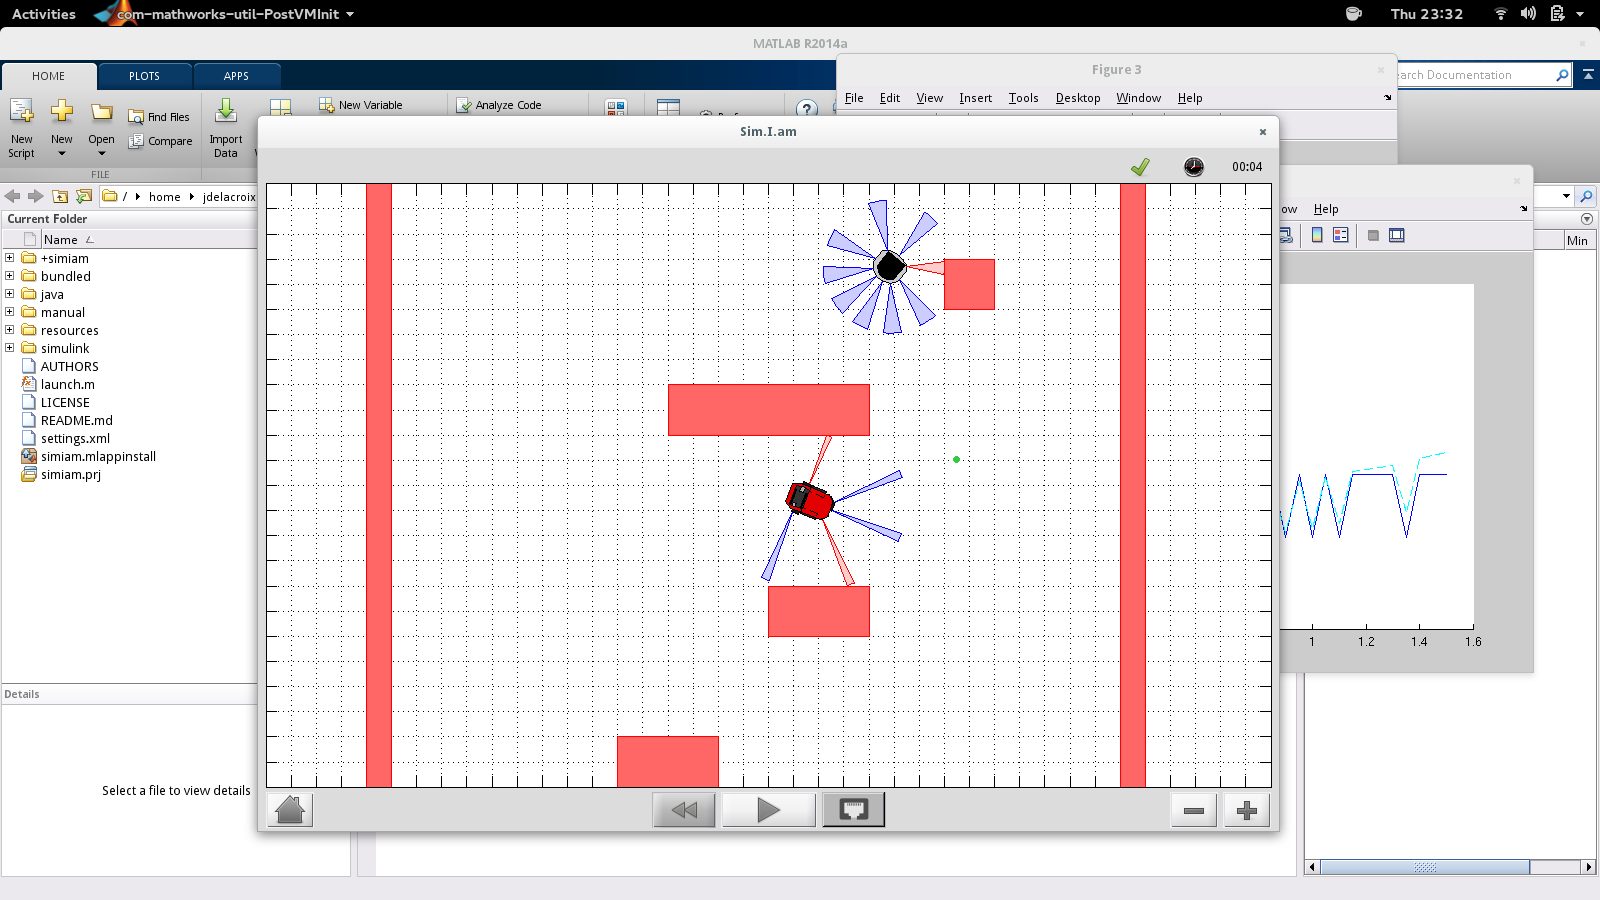
\includegraphics[trim={0cm 0cm 0cm 0cm},clip,
scale=0.16]{Figuras/simiam-screenshot}
	
	%\textbf{Fonte: \citeonline{im:Simiam}}
\end{figure}
\end{frame}

\begin{frame}
	\begin{exampleblock}{Alterações mais importantes}
		\begin{itemize}
		  \item Incluir uma classe para implementar aspectos físicos do robô deste
		  trabalho.
		  \item Incluir suporte para controladores \textit{fuzzy}.
		\end{itemize}
	\end{exampleblock}
\end{frame}

\subsection{Considerações Finais}
\begin{frame}
	\frametitle{Considerações Finais}
	
	\begin{block}{}
		\begin{itemize}
		  \item Autonomia em arquiteturas não deliberativas.
		  \item Estimativa de estado.
		  \item Comparação qualitativa.
		\end{itemize}
	\end{block}
\end{frame}

\subsection{Agradecimentos}
\begin{frame}
	%\frametitle{Obrigado pela presença!}
	\titlepage
\end{frame}

\end{document}